\documentclass[11pt]{article}
\usepackage[utf8]{inputenc}	% Para caracteres en español
\usepackage{amsmath,amsthm,amsfonts,amssymb,amscd}
\usepackage{multirow,booktabs}
\usepackage[table]{xcolor}
\usepackage{fullpage}
\usepackage{lastpage}
\usepackage{enumitem}
\usepackage{fancyhdr}
\usepackage{mathrsfs}
\usepackage{wrapfig}
\usepackage{setspace}
\usepackage{calc}
\usepackage{multicol}
\usepackage{cancel}
\usepackage[retainorgcmds]{IEEEtrantools}
\usepackage[margin=1cm]{geometry}
\usepackage{amsmath}
\newlength{\tabcont}
\setlength{\parindent}{0.0in}
\setlength{\parskip}{0.05in}
\usepackage{empheq}
\usepackage{framed}
\usepackage[most]{tcolorbox}
\usepackage{xcolor}
\usepackage{graphicx}
\usepackage{listings}
% -- Basic formatting
\usepackage[utf8]{inputenc}
\usepackage[english]{babel}
\usepackage{times}
\usepackage{caption}
\usepackage{subcaption}
\usepackage{placeins}
\setlength{\parindent}{0pt}
\usepackage{indentfirst}% -- Defining colors:
\usepackage[dvipsnames]{xcolor}
\definecolor{codegreen}{rgb}{0,0.6,0}
\definecolor{codegray}{rgb}{0.5,0.5,0.5}
\definecolor{codepurple}{rgb}{0.58,0,0.82}
\definecolor{backcolour}{rgb}{0.95,0.95,0.92}% Definig a custom style:
\lstdefinestyle{mystyle}{
    backgroundcolor=\color{backcolour},   
    commentstyle=\color{codepurple},
    keywordstyle=\color{NavyBlue},
    numberstyle=\tiny\color{codegray},
    stringstyle=\color{codepurple},
    basicstyle=\ttfamily\footnotesize\bfseries,
    breakatwhitespace=false,         
    breaklines=true,                 
    captionpos=t,                    
    keepspaces=true,                 
    numbers=left,                    
    numbersep=5pt,                  
    showspaces=false,                
    showstringspaces=false,
    showtabs=false,                  
    tabsize=2
}% -- Setting up the custom style:
\lstset{style=mystyle}
\lstset{
  style=mystyle,
  framexleftmargin=3.5mm,
  rulesepcolor=\color{black},
  linewidth=0.6\linewidth,
  xleftmargin=12pt,
  aboveskip=12pt,
  belowskip=12pt
}
\colorlet{shadecolor}{orange!15}
\parindent 0in
\parskip 1pt
\geometry{margin=1in, headsep=0.25in}
\theoremstyle{definition}
\newtheorem{defn}{Definition}
\newtheorem{reg}{Rule}
\newtheorem{exer}{Exercise}
\newtheorem{note}{Note}
\graphicspath{ {./images/} }
\begin{document}
\setcounter{section}{0}
\title{MIE223 Lecture Notes}

\thispagestyle{empty}

\begin{center}
{\LARGE \bf Data Cleaning}\\
{\large MIE223}\\
Winter 2025
\end{center}
\section{Why Clean Data?}
\subsection{Example}
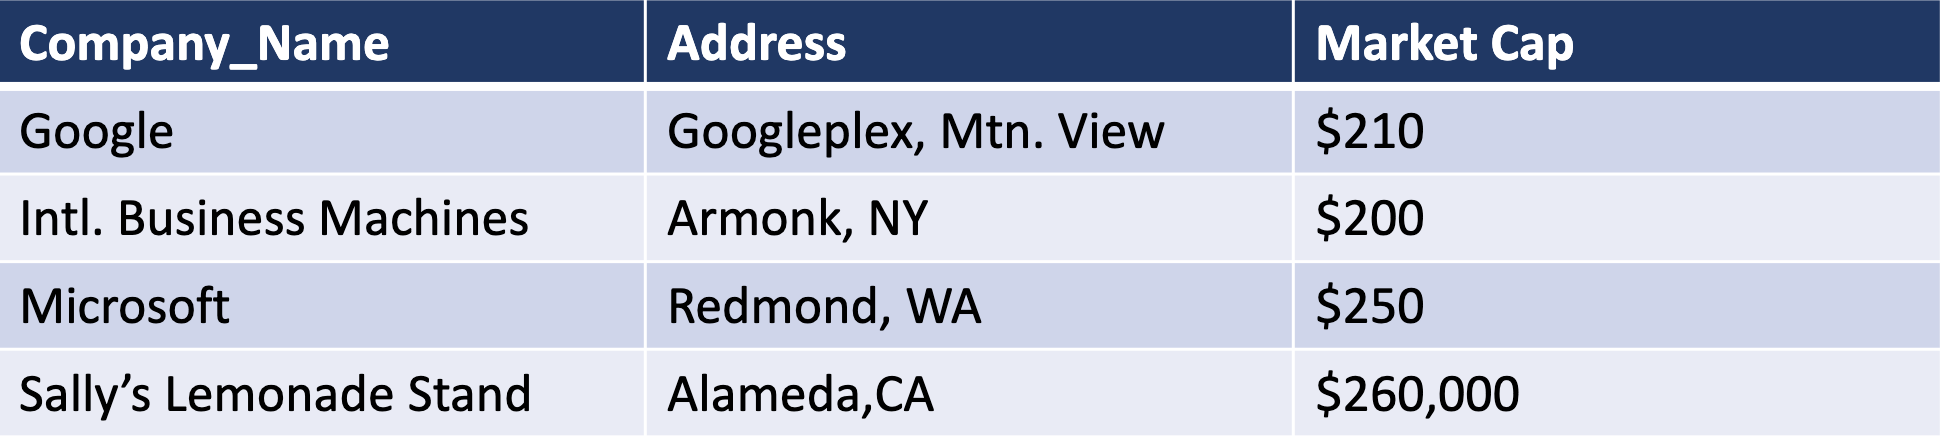
\includegraphics[width=\textwidth]{1.png}
\begin{itemize}
    \item Apple: Missing Data
    \item IBM: Entity Resolution / Unnormalized Naming
    \item Sally's Lemonade Stand: Unit Mismatch
\end{itemize}
\subsection{Where is Data Cleaning in the Organization?}
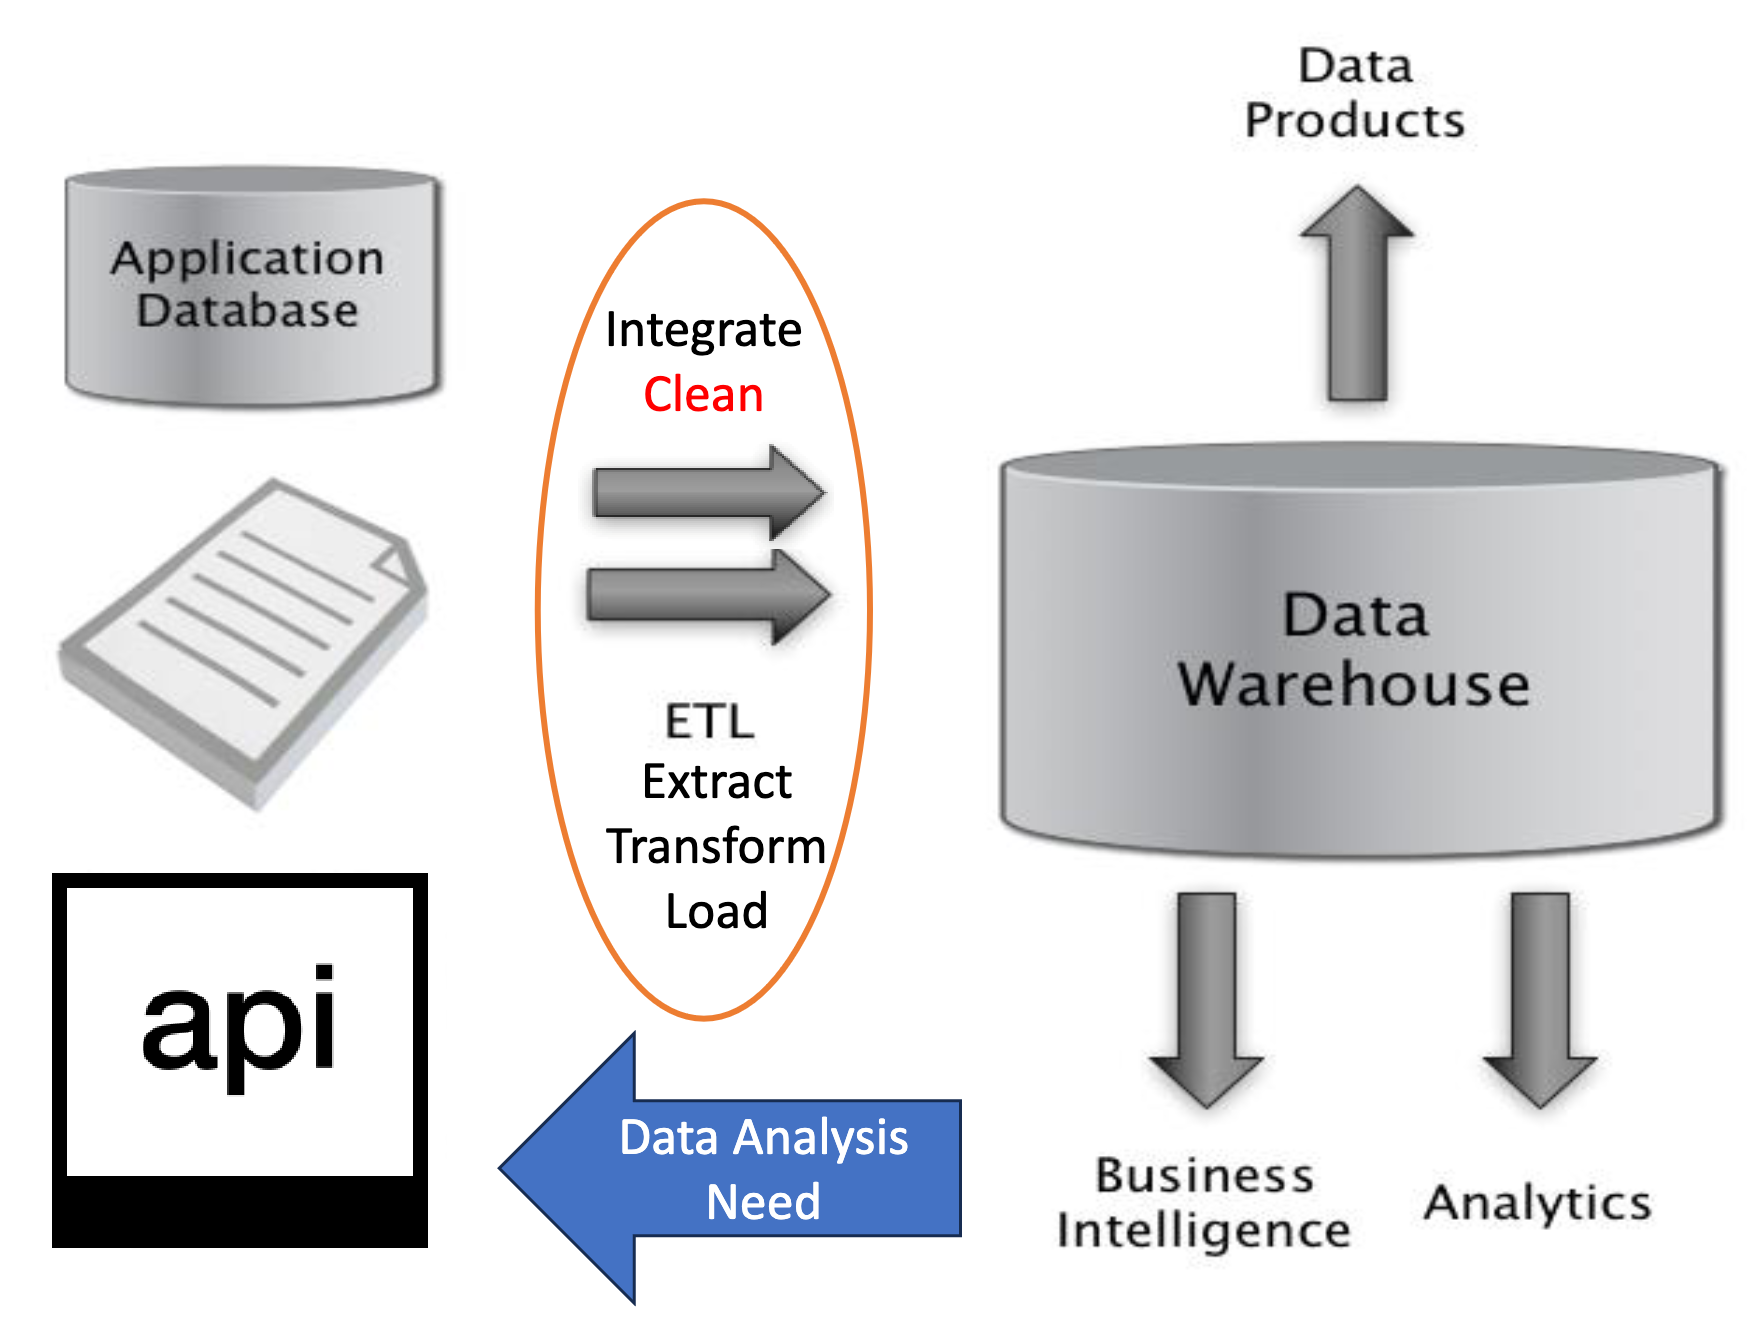
\includegraphics[width=\textwidth/2]{2.png}
\begin{itemize}
    \item Data comes in all shapres and forms
    \item ETL: Extract, Transform, Load
    \item Data science exists in business intelligence and analytics
    \item Data engineers work in application database
\end{itemize}
\subsection{Cost of Bad Quality Data Over Time}
\begin{itemize}
    \item Cost for preventing bad data: \$1
    \item Cost for correcting bad data: \$10
    \item Cost for fixing problem resulting from bad data: \$100
\end{itemize}

\section{Perspectives on Data Science
and Data Cleaning}
\subsection{Data Science is an Intersectional Discipline}
\begin{itemize}
    \item Computer Science
    \item Math and Statistics
    \item Domain Knowledge
\end{itemize}
\subsection{Dirty Data}
\begin{itemize}
    \item The Statistics View:
    \begin{itemize}
        \item There is a process that produces data
        \item Any dataset is a sample of the output of that process
        \item Results are probabilistic
        \item You can correct bias in your sample
    \end{itemize}
    \item The Database View:
    \begin{itemize}
        \item I got my hands on this data set
        \item Some of the values are missing, corrupted, wrong, duplicated
        \item Results are absolute (relational model)
        \item You get a better answer by improving the quality of the values in your dataset
    \end{itemize}
    \item The Domain Expert’s View
    \begin{itemize}
        \item This Data Doesn’t look right
        \item This Answer Doesn’t look right
        \item What happened?
    \end{itemize}
    \item The data scientist's view is a combination of the above.
\end{itemize}
\begin{note}
    A Data scientist knows more programming than a statistician
    and more statistics than a programmer.
    A Data scientist intimately understands their domain!
\end{note}
\subsection{Data Quality Problems}
\begin{itemize}
    \item Data is dirty on its own
    \begin{itemize}
        \item Human collection or data entry (generally lazy and want to see their children)
    \end{itemize}
    \item Data sets are clean but integration (i.e., combining them)
    screws them up (such as different units of measurement)
    \item Data sets are clean but suffer “bit rot” (lose data from cutting)
    \begin{itemize}
        \item Constant data transformations introduce errors, noise, data loss
        \item Meanings of labels change over time
    \end{itemize}
    \item Any combination of the above... and much, much more!
\end{itemize}
\subsection{Some Data Issues you will Encounter}
\begin{enumerate}
    \item Parsing text into fields (separator issues)
    \item Naming conventions and entity resolution D: NYC vs New York
    \item Missing required field (birthdate)
    \item Gaps in time series
    \item Different representations (“2” vs 2), Unicode lookalikes
    \item Fields too long (get truncated)
    \item Mixed data types (feet, meters)
    \item Redundant Records (exact match or other)
    \item Formatting issues – especially dates
    \item Licensing issues/privacy/cost prevent access to all data
\end{enumerate}
\subsection{Key Types of Data Quality Issues}
\begin{itemize}
    \item \textbf{incomplete}: lacking attribute values, lacking certain attributes
    of interest, or containing only aggregate data
    \begin{itemize}
        \item e.g., occupation=“ ”
    \end{itemize}
    \item \textbf{noisy}: containing errors or outliers
    \begin{itemize}
        \item e.g., Salary=“-10”
    \end{itemize}
    \item \textbf{inconsistent}: containing discrepancies in codes or names
    \begin{itemize}
        \item e.g., Age=“42” Birthday=“03/07/1997”
        \item e.g., Was rating “1,2,3”, now rating “A, B, C”
        \item e.g., discrepancy between duplicate records
    \end{itemize}
    \item \textbf{redundancy}: duplicated content
\end{itemize}
\subsection{Why Is Data Dirty?}
\begin{itemize}
    \item Incomplete data may come from
    \begin{itemize}
        \item “Not applicable” data value when collected
        \item Changes in the data collected over time
        \item Human/hardware/software problems
    \end{itemize}
    \item Noisy data (incorrect values) may come from
    \begin{itemize}
        \item Faulty data collection instruments, undocumented API changes
        \item Human or computer error at data entry, UI changes!
        \item Errors in data transmission, discretization, conversion (losing precision)
        \item Typing errors (meters, feet, km mixed in same column)
    \end{itemize}
    \item Inconsistent data may come from
    \begin{itemize}
        \item Different data sources (data integration)
        \item Changes in data collection practices over time
    \end{itemize}
    \item Redundancy
    \begin{itemize}
        \item Human error (could not find previous record), data integration
    \end{itemize}
\end{itemize}
\section{The Role of Data Cleaning in
Data Science}
\subsection{Data Science in the Real World}
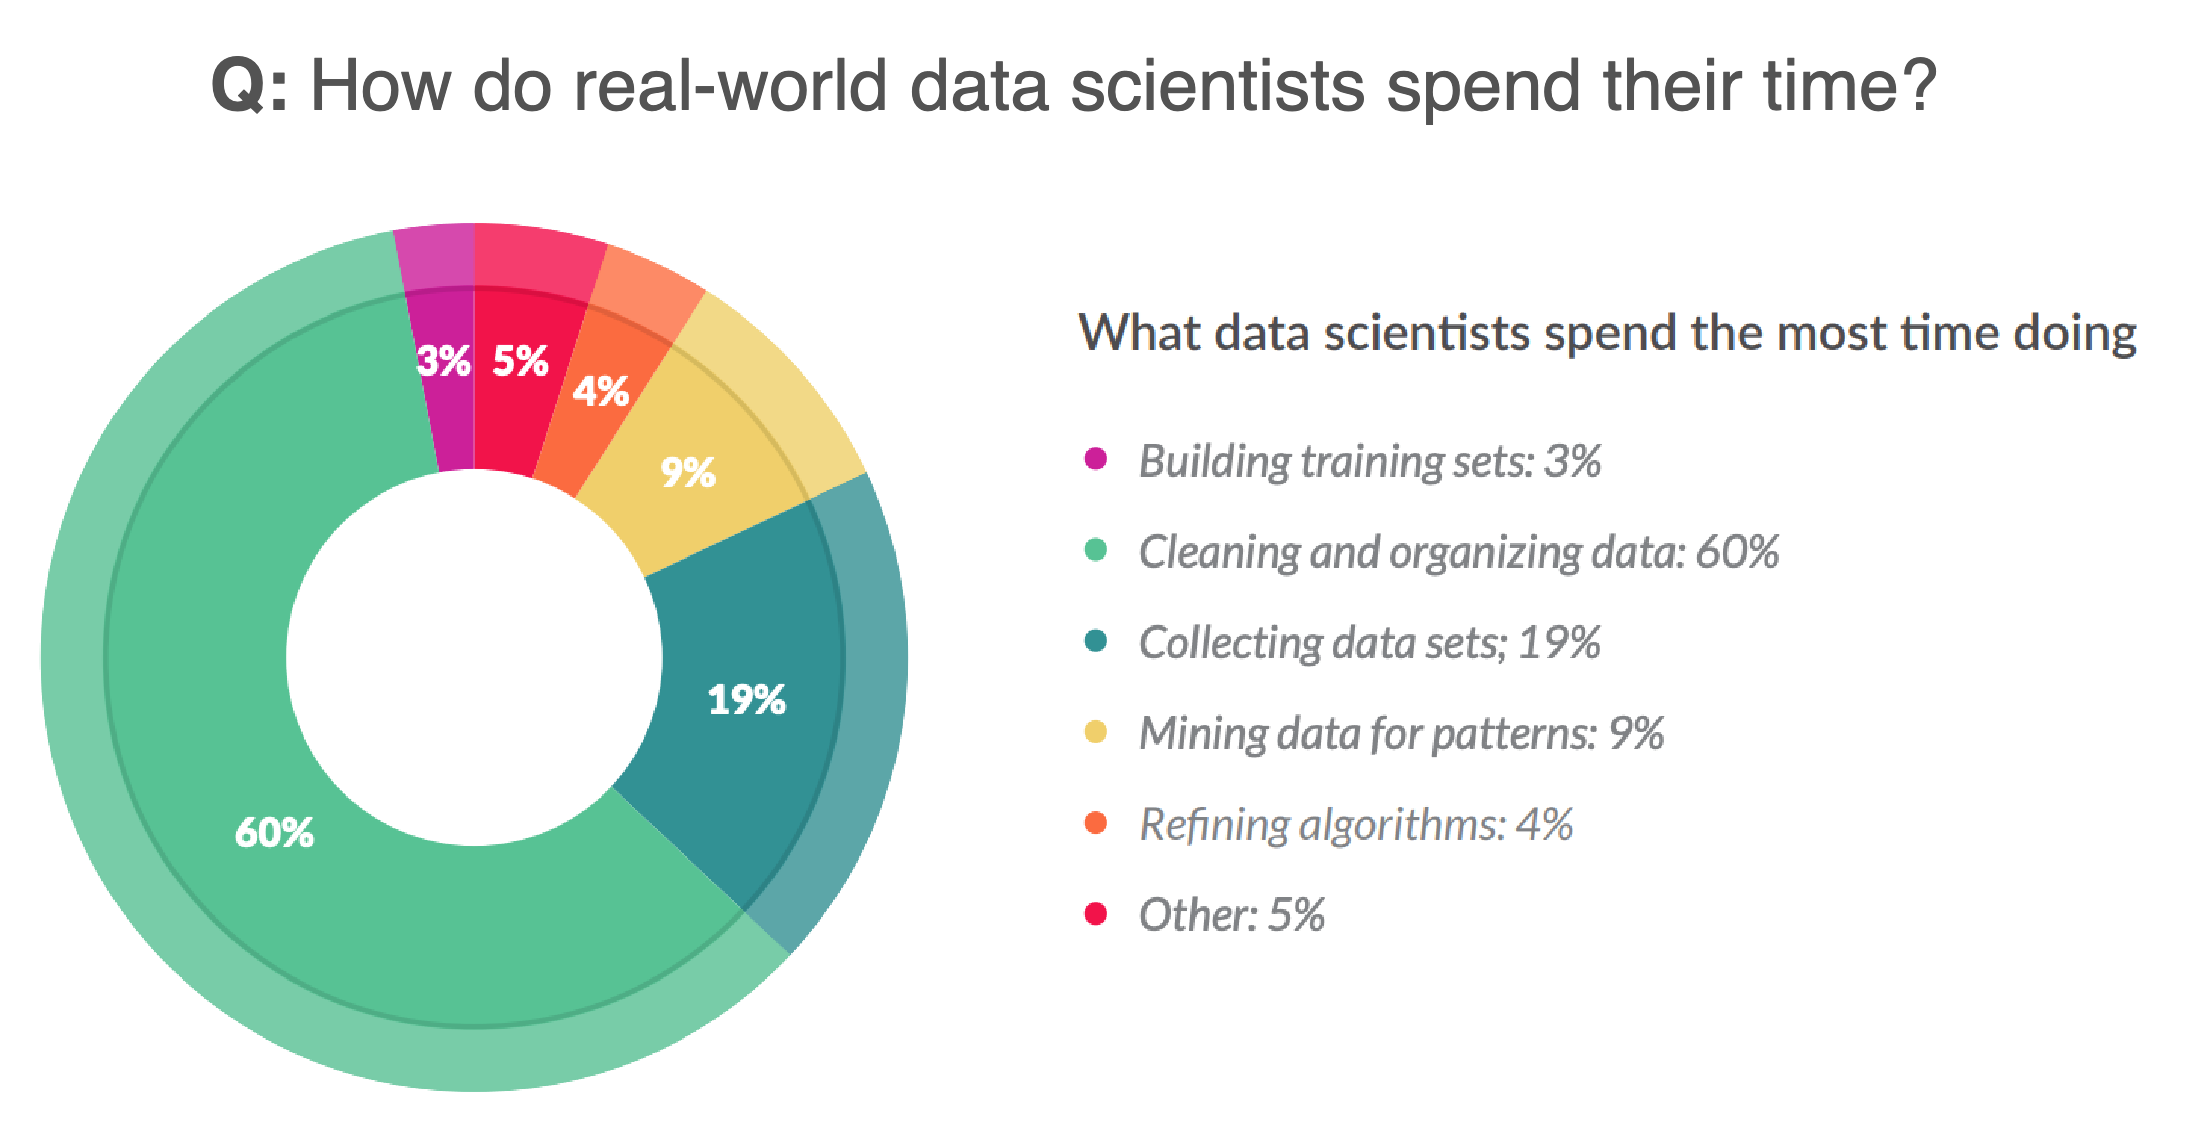
\includegraphics[width=\textwidth]{3.png}


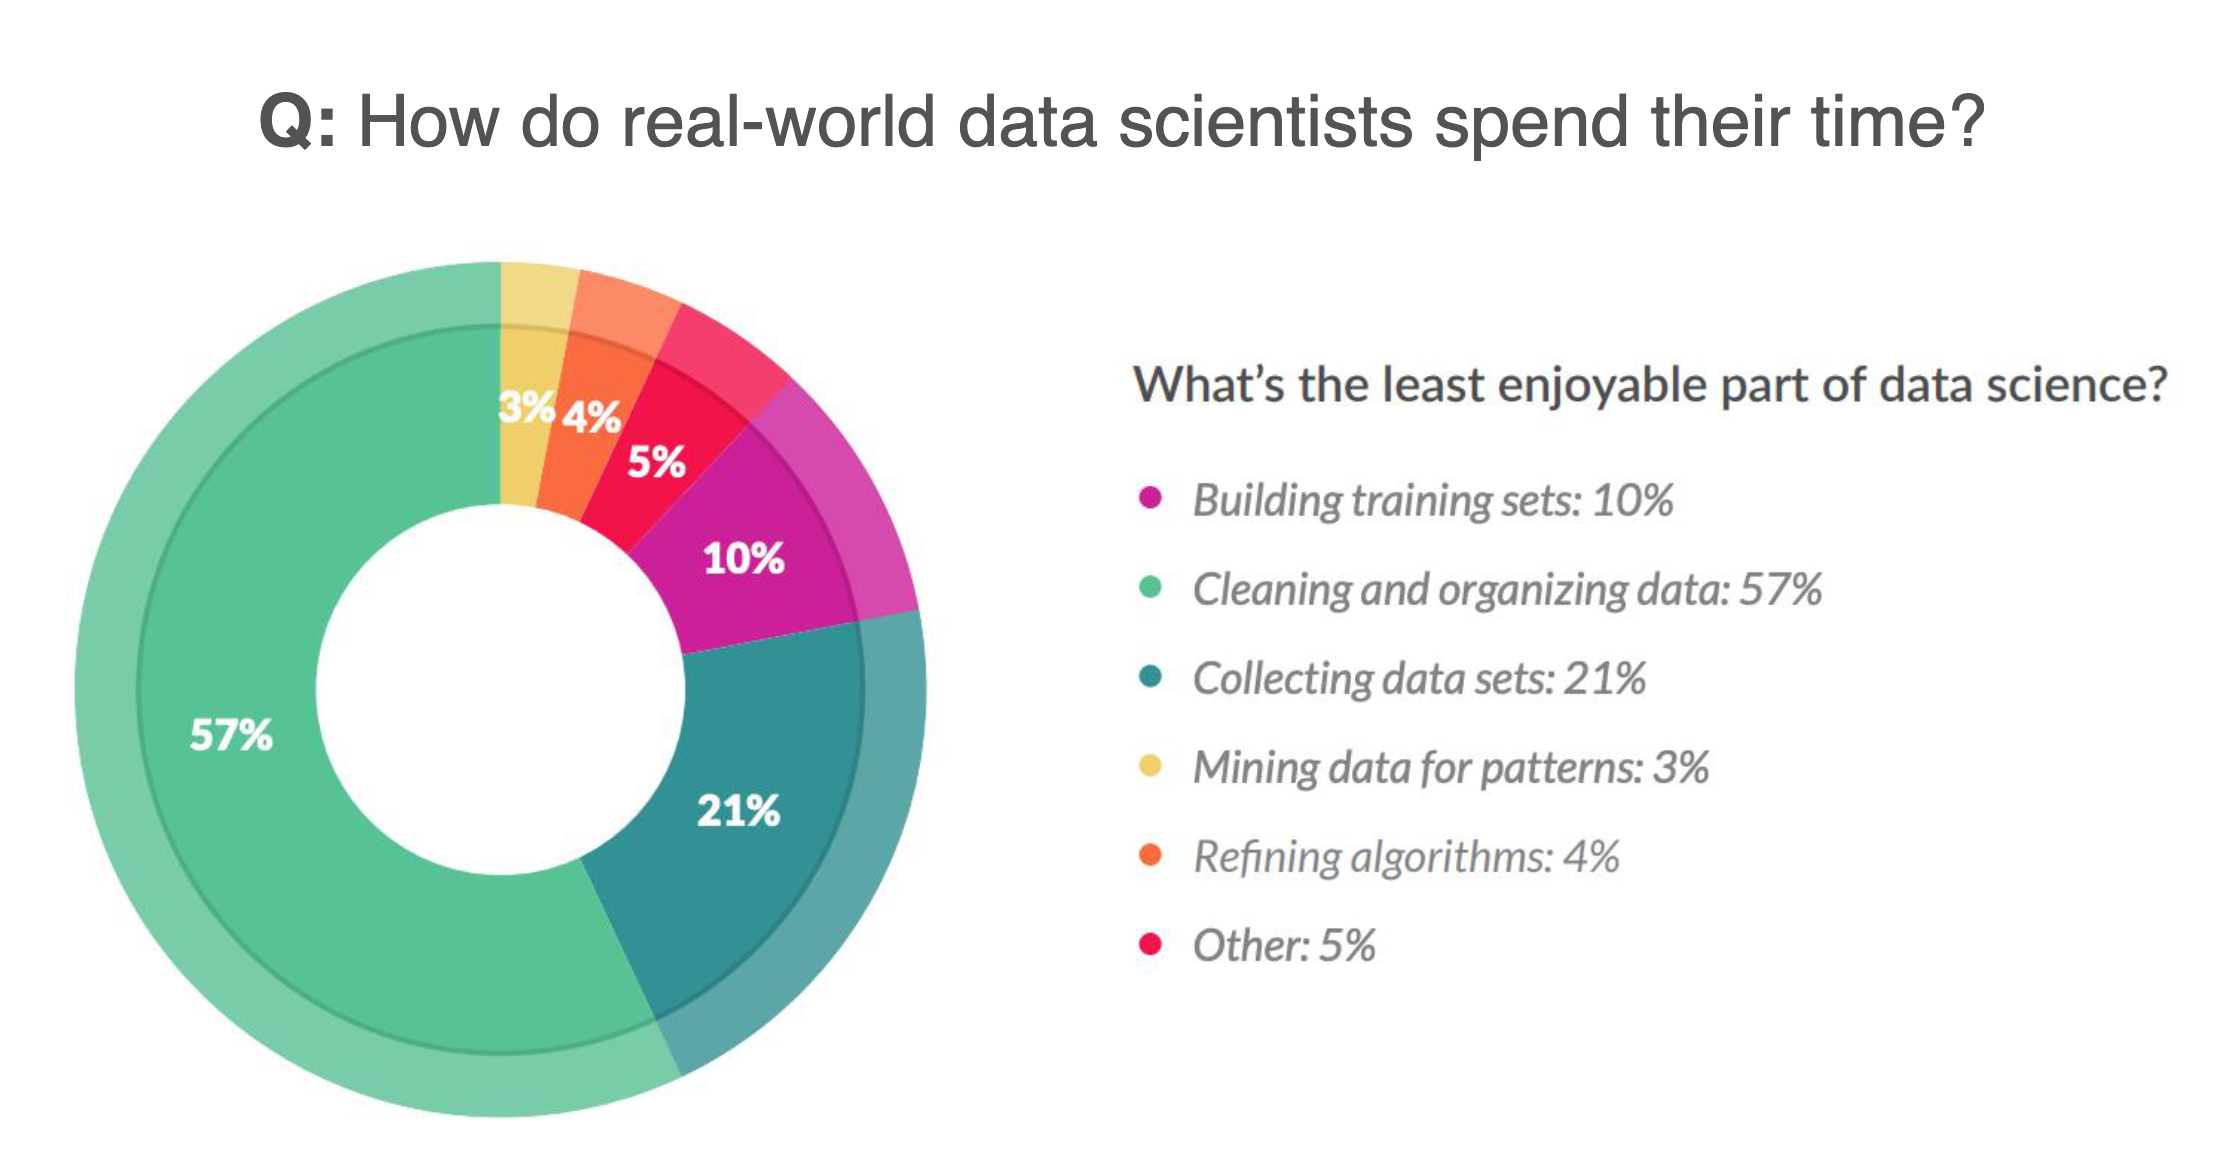
\includegraphics[width=\textwidth]{4.png}
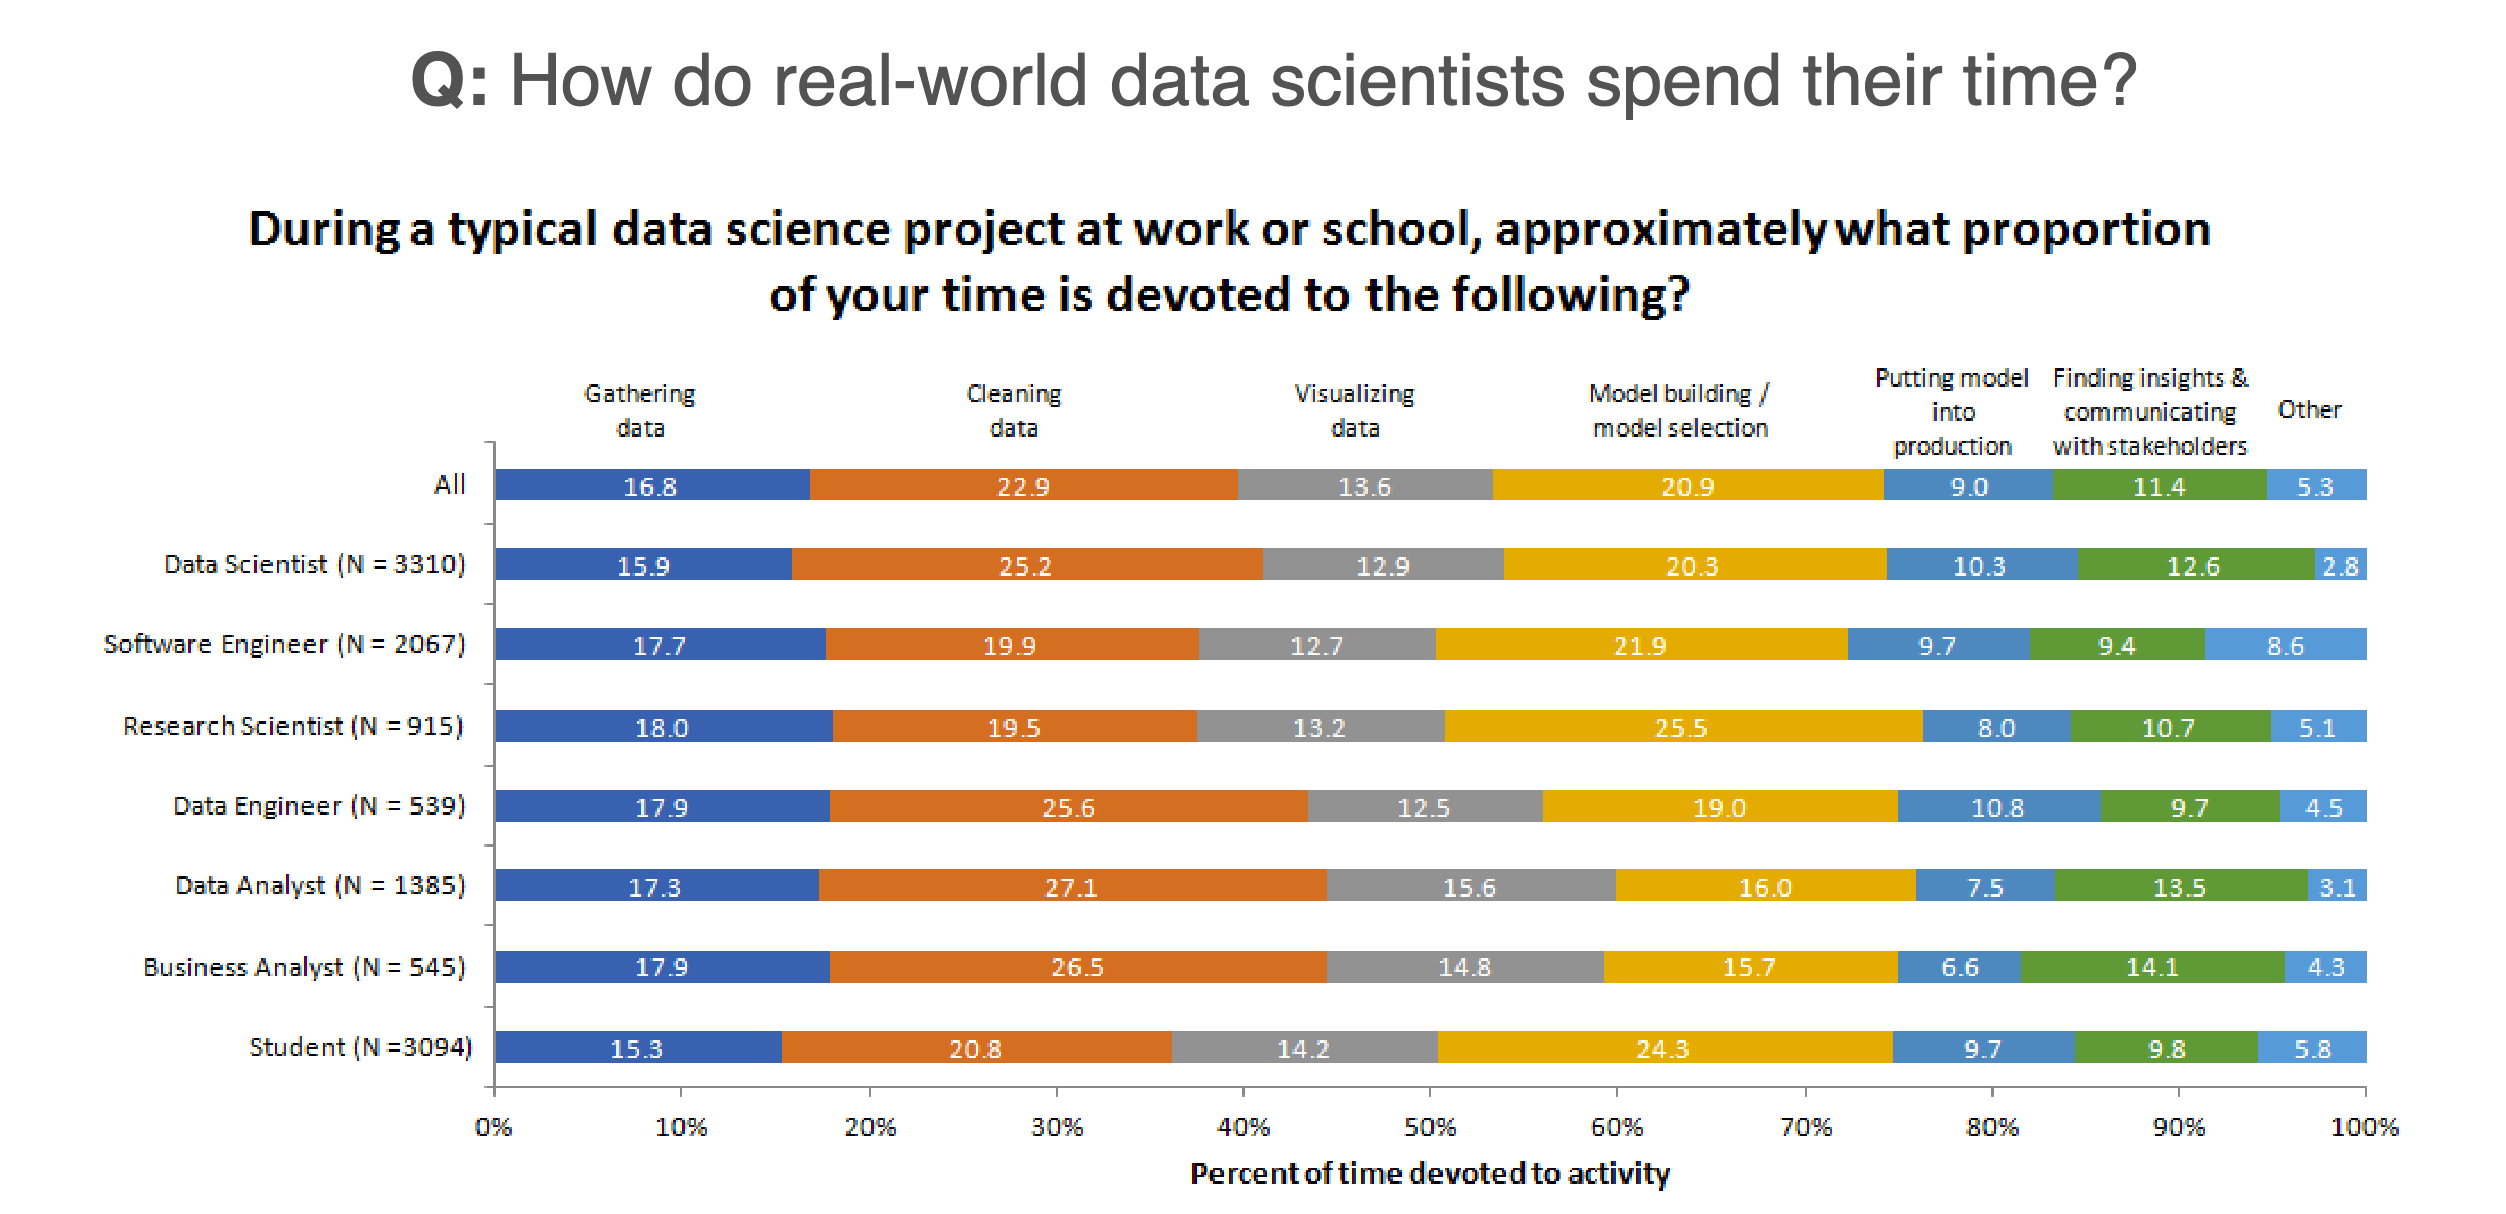
\includegraphics[width=\textwidth]{5.png}
\subsection{Data Cleaning Makes Everything Okay?}
\begin{note}
    “The appearance of a hole in the
earth's ozone layer over
Antarctica, first detected in 1976,
was so unexpected that scientists
didn't pay attention to what their
instruments were telling them;
they thought their instruments
were malfunctioning.”
- National Center for
Atmospheric Research
\end{note}
The data was rejected as unreasonable by data quality control algorithms.
% 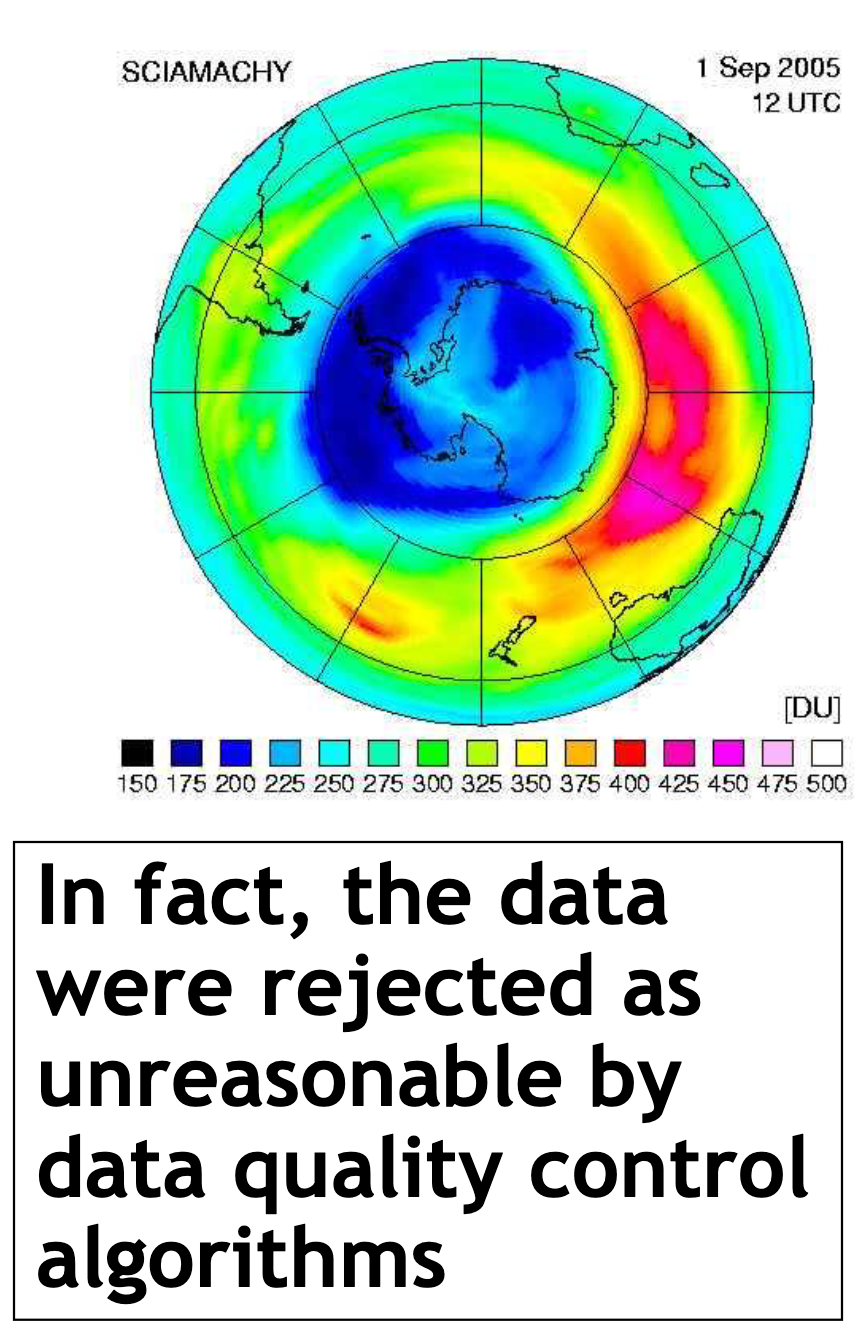
\includegraphics[width=\textwidth/3]{6.png}
\section{Principles of Data Cleaning}
\subsection{Data Cleaning Tasks}
\begin{itemize}
    \item Data Summary
    \item Consider filling in missing values
    \item Identify outliers and smooth out noisy data
    \item Correct inconsistent data
    \item Resolve redundancy
\end{itemize}
\section{Data Cleaning: Data Summary}
\subsection{Data Summary Procedure}
\begin{itemize}
    \item Look at data types of columns
    \begin{itemize}
        \item Beware of "Object" columns, indicator that you've mixed types (e.g., "2" and 2)
    \end{itemize}
    \item For high cardinality strings and categorical (e.g,. "country") columns
    \begin{itemize}
        \item How many unique elements are there?
        \item Are any missing?
        \item Count frequencies of string
        \begin{itemize}
            \item Look at top-10 most frequent and least frequent values
            \item Look at strings near the mean and median frequency
        \end{itemize}
    \end{itemize}
    \item For low cardinality strings and categorical (e.g,. “province") columns
    \begin{itemize}
        \item Look at frequency of each unique value
    \end{itemize}
    \item For ordinal numeric (integers) or floating point values
    \begin{itemize}
        \item Compute summary statistics
        \item View a histogram (but before you do this, hypothesize what you will see)
    \end{itemize}
\end{itemize}
\subsection{Summary Statistics and for Each Variable (Column)}
\begin{itemize}
    \item Range
    \begin{itemize}
        \item Minimum
        \item Maximum
    \end{itemize}
    \item Central Tendency
    \begin{itemize}
        \item Mean
        \item Median
        \item Mode
        \begin{itemize}
            \item Value that occurs most frequently in discrete data
            \item Value with highest probability in continuous data
            \item Informally: \# peaks in numeric data – unimodal, bimodal, trimodal, multimodal, ...
        \end{itemize}
    \end{itemize}
    \item If Data is non-numeric, consider frequencies below (e.g., mean frequency of jobs in “Job”)
    \item If Data is a string, consider sorting it and looking at nearby values
\end{itemize}
\subsection{Measuring the Dispersion of Data}
\begin{itemize}
    \item Quartiles, outliers and boxplots
    \begin{itemize}
        \item Quartiles: Q1 (25th percentile), Q3 (75th percentile)
        \item Inter-quartile range: IQR = Q3 – Q1
        \item Five number summary: min, Q1, M, Q3, max
        \item Boxplot: ends of the box are the quartiles, median is marked, whiskers (min / max),
        and plot outlier individually
        \item Outlier: usually, a value higher/lower than 1.5 x IQR
    \end{itemize}
    \item Variance and standard deviation (sample: s, population: sigma)
    \begin{itemize}
        \item Variance: (algebraic, scalable computation)
        \item 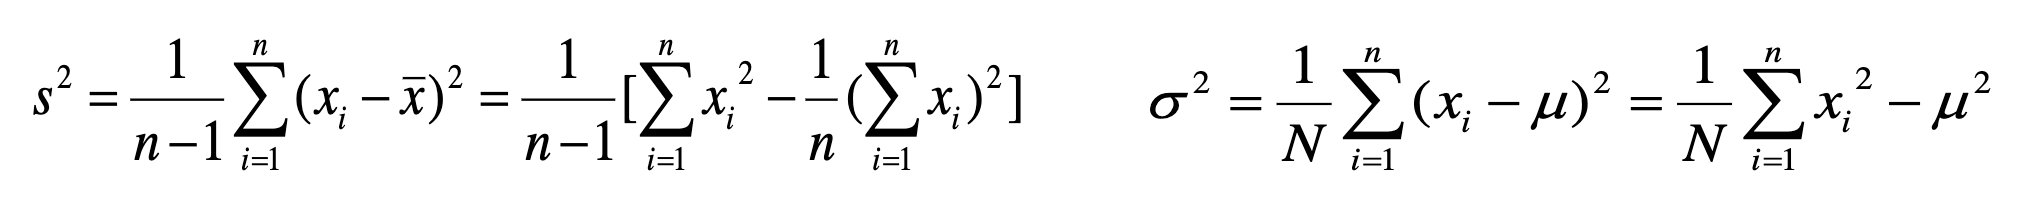
\includegraphics[width=\textwidth]{7.png}
        % \item Standard deviation s (or sigma) is the square root of variance s^2 (or sigma^2)
    \end{itemize}
\end{itemize}
\end{document}